\chapter{Specifikacija programske potpore}
		
	\section{Funkcionalni zahtjevi}
	\bigskip
		
			\noindent \textbf{Dionici:}
			
			\begin{packed_enum}
				
				\item Klijent
				\item Klub
				\item Trener
				\item Administrator
				\item Razvojni tim
				
			\end{packed_enum}
		\bigskip
		\bigskip
	
		
			
			\noindent \textbf{Aktori i njihovi funkcionalni zahtjevi:}
			\bigskip
		
			\begin{packed_enum}
				\item  \underbar{Neregistrirani/neprijavljeni korisnik (inicijator) može:}
				
				\begin{packed_enum}
					
					\item pregledati profil kluba i tipove plesova koje klub nudi
					\item pregledati karte dostupnih plesnjaka i lokacije klubova
					\item filtrirati plesnjake po:
					\begin{packed_enum}
						
						\item  tipu plesa
						\item  klubu organizatoru i tipu plesa
				
					\end{packed_enum}
					\item  filtrirati klubove po tipovima plesa za koje organiziraju tečaj
					\item kreirati račun (korisničko ime, lozinka, prezime, spol, datum rođenja, broj mobitela, email adresa, opcionalno opis plesnog iskustva i fotografija)
						
				\end{packed_enum}
			\bigskip
			\bigskip
			\bigskip
			\bigskip
			\bigskip
			\bigskip
			\bigskip
			\bigskip
			\bigskip
			

				\item \underbar{Klijent (inicijator) može:}
				
				\begin{packed_enum}
					\item pregledati i izmijeniti osobne podatke
					\item obrisati korisnički račun
					\item prikazati tečajeve slobodne za upis, na karti:
					\begin{packed_enum}
						\item rezultate filtrirati po vremenu održavanja i tipu plesa
					\end{packed_enum}
					\item odabrati tečaj (vrsta plesa, kalendar održavanja, ime i prezime te slika trenera)
					\item klubu poslati prijavu da postane trener:
					\begin{packed_enum}
						\item postavi motivacijsko pismo
						\item postavi pdf datoteku potvrde da je sposoban držati tečaj
					\end{packed_enum}
					\item pregledati aktivne prijave na tečaj nekog kluba
					\item prijaviti se na tečaj kluba
					\item poslati zahtjev za otvaranje kluba
				\end{packed_enum}
			\bigskip
			\bigskip
				
				\item \underbar{Administrator (inicijator) može:}
				\begin{packed_enum}
					\item potvrditi nove registrirane klubove
					\item dodavati, mijenjati i brisati plesove
					\item pregledati popise svih klijenata i klubova
					\item uređivati korisničke račune
				\end{packed_enum}
			\bigskip
			\bigskip
				
				\item \underbar{Vlasnik kluba (inicijator) može:}
				\begin{packed_enum}	
					\item raditi sve isto kao i klijent
					\item pregledati i izmijeniti osobne podatke kluba 
					\item obrisati korisnički račun kluba 
					\item organizirati plesnjak (lokacija, naziv, opis i slika, tipovi plesa)
					\item potvrditi klijentovu prijavu za trenera
					\item prikazati informacije:
					\begin{packed_enum}
						\item ime kluba, kontakt telefon, email adresa, kratki opis kluba
						\item popis plesova koje njihovi treneri izvode
						\item prikaz lokacija plesova i dvorana na karti
					\end{packed_enum}
					\item postaviti poveznicu na stranicu s grupama za upis
					\item objaviti upis za tečaj s vremenskim rokom
					\item odabrati klijente koji se primaju u grupu
					\item mijenjati popis klijenata
					\item urediti ili brisati grupe
				\end{packed_enum}
			\bigskip
			\bigskip
				
				\item \underbar{Baza podataka (sudionik) može:}
				\begin{packed_enum}
					\item pohraniti podatke o korisnicima i njihovim ovlasitima
					\item pohraniti podatke o klubovima, plesovima koje oni nude, tečajevima, dvoranama i lokacijama odvijanja
				\end{packed_enum}
			\bigskip
			\bigskip
				
				\item \underbar{Trener (inicijator) može:}
				\begin{packed_enum}
					\item raditi sve isto kao i klijent
					\item pregledati popis grupa koje trenira
					\item pregledati termine tečajeva koje vodi na kalendaru
					\item pregledati popise klijenata koji bi trebali biti nazočni
				\end{packed_enum}
					
				%\item  \underbar{Grupa (inicijator) može:}
				
			%	\begin{packed_enum}
					
				%	\item pregledati podatke o treneru
				%	\item pregledati skup treninga kroz neki vremenski period
				%	\item pregledati maksimalan broj sudionika
				%	\item dati informaciju o težini treninga
				%	\item postaviti uvjete treniranja, pravila ponašanja
					
				%\end{packed_enum}
			\end{packed_enum}
			
			\eject 
			
			
				
			\subsection{Obrasci uporabe}
				

				\subsubsection{Opis obrazaca uporabe}
					\textit{ Obrasci uporabe (Use Cases) numerirani su oznakama od UC1 do UC32, pomoću njih opisujemo tipičnu uporabu sustava.}\\
				
					\noindent \underbar{\textbf{UC1 - Pregled klubova}}
					\begin{packed_item}
						
						\item \textbf{Glavni sudionik: Neregistrirani korisnik, klijent}
						\item  \textbf{Cilj: Pregled klubova} 
						\item  \textbf{Sudionici: Baza podataka}
						\item  \textbf{Preduvjet: -}
						\item  \textbf{Opis osnovnog tijeka: }
						
						\item[] \begin{packed_enum}
							
							\item Karta je prikazana prilikom učitavanja aplikacije
							\item Neregistrirani korisnik/klijent na karti vidi lokacije klubova te odabire klub
							\item Prikazuju se informacije o klubu, tečajevima te plesnjacima
							
						\end{packed_enum}
				\end{packed_item}
			
					\noindent \underbar{\textbf{UC2 - Registracija korisnika}}
					\begin{packed_item}
						
						\item \textbf{Glavni sudionik: Neregistrirani korisnik}
						\item  \textbf{Cilj: Stvoriti korisnički račun za pristup sustavu} 
						\item  \textbf{Sudionici: Baza podataka}
						\item  \textbf{Preduvjet: -}
						\item  \textbf{Opis osnovnog tijeka: }
						
						\item[] \begin{packed_enum}
							
							\item Neregstrirani korisnik odabire opciju za registraciju
							\item Neregistrirani korisnik unosi sve potrebne informacije kako bi se registrirao
							\item Klijentu se prikazuju informacije početne stranice
							
						\end{packed_enum}
						
						\item  \textbf{Opis mogućih odstupanja:}
						
						\item[] \begin{packed_item}
							
							\item[2.a] Unos podataka u neispravnom formatu, email ili korisničko ime koje je već korišteno od strane drugog klijenta, email ili korisničko ime koje nije registrirano
							\item[] \begin{packed_enum}
								
								\item Sustav obaviještava neregistriranog korisnika o grešci te ga vraća opet na stranicu za registraciju
								\item Neregistrirani korisnik unosi ispravne podatke te se uspješno registrira ili odustaje od registracije
								
							\end{packed_enum}
							
							
							
						\end{packed_item}
						
					\end{packed_item}
				
					\noindent \underbar{\textbf{UC3 - Prijava u sustav}}
					\begin{packed_item}
						
						\item \textbf{Glavni sudionik: Klijent}
						\item  \textbf{Cilj: Dobiti pristup korisničkom sučelju} 
						\item  \textbf{Sudionici: Baza podataka}
						\item  \textbf{Preduvjet: prethodna registracija}
						\item  \textbf{Opis osnovnog tijeka: }
						
						\item[] \begin{packed_enum}
							
							\item Unos korisničkog imena i lozinke
							\item Potvrda o ispravnosti unesenih podataka
							\item Pristup klijentskim funkcijama
							
						\end{packed_enum}
						
						\item  \textbf{Opis mogućih odstupanja:}
						
						\item[] \begin{packed_item}
							
							\item[2.a] Neispravno uneseno korisničko ime ili lozinka
							\item[] \begin{packed_enum}
								
								\item Sustav obaviještava klijenta te ga vraća na stranicu za prijavu
								
							\end{packed_enum}
							
						\end{packed_item}
						
					\end{packed_item}
				
					\noindent \underbar{\textbf{UC4 - Pregled osobnih podataka}}
					\begin{packed_item}
						
						\item \textbf{Glavni sudionik: Klijent}
						\item  \textbf{Cilj: Pregledati osobne podatke} 	
						\item  \textbf{Sudionici: Baza podataka}
						\item  \textbf{Preduvjet: Klijent je prijavljen u sustav}
						\item  \textbf{Opis osnovnog tijeka: }
						
						\item[] \begin{packed_enum}
							
							\item Klijent odabire opciju "Osobni podatci"
							\item Aplikacija prikazuje osobne podatke klijenta
						\end{packed_enum}
					
				\end{packed_item}
						
					\noindent \underbar{\textbf{UC5 - Promjena osobnih podataka}}
					\begin{packed_item}
							
						\item \textbf{Glavni sudionik: Klijent}
						\item  \textbf{Cilj: Promijeniti osobne podatke} 
						\item  \textbf{Sudionici: Baza podataka}
						\item  \textbf{Preduvjet: Klijent je prijavljen u sustav}
						\item  \textbf{Opis osnovnog tijeka: }
							
						\item[] \begin{packed_enum}
								
							\item Klijent odabire opciju za promjenu osobnih podataka
							\item Klijent unosi nove podatke te ih sprema
							\item Baza podataka se ažurira
						\end{packed_enum}
							
						\item  \textbf{Opis mogućih odstupanja:}
							
						\item[] \begin{packed_item}
								
							\item[2.a] Klijent unosi nove podatke, ali ih ne sprema
							\item[] \begin{packed_enum}
									
								\item Aplikacija obaviještava klijenta da mora spremiti promijenjene podatke
									
							\end{packed_enum}
								
						\end{packed_item}
							
					\end{packed_item}
					
					\noindent \underbar{\textbf{UC6 - Brisanje korisničkog računa}}
					\begin{packed_item}
						
						\item \textbf{Glavni sudionik: Klijent}
						\item  \textbf{Cilj: Izbrisati svoj korisnički račun} 
						\item  \textbf{Sudionici: Baza podataka}
						\item  \textbf{Preduvjet: Klijent je prijavljen u sustav}
						\item  \textbf{Opis osnovnog tijeka: }
						
						\item[] \begin{packed_enum}
							
							\item Klijent pregledava osobne podatke
							\item Otvara se stranica sa osobnim podatcima klijenta
							\item Klijent briše korisnički račun
							\item Korisnički račun se briše iz baze podataka
							\item Otvara se početna stranica
						\end{packed_enum}
						
						
					\end{packed_item}
				\bigskip
					\bigskip
						\bigskip
					
						\noindent \underbar{\textbf{UC7 - Prikaz  tečajeva}}
						\begin{packed_item}
							
							\item \textbf{Glavni sudionik: Klijent}
							\item  \textbf{Cilj: Prikazati tečajeve slobodne za upis na karti} 
							\item  \textbf{Sudionici: Baza podataka}
							\item  \textbf{Preduvjet: Klijent je prijavljen u sustav }
							\item  \textbf{Opis osnovnog tijeka: }
							
							\item[] \begin{packed_enum}
								
								\item Klijentu se na karti prikazuje popis  tečajeva
							\end{packed_enum}
							\bigskip
								\bigskip
									\bigskip
							
							
						\end{packed_item}
					
						\noindent \underbar{\textbf{UC8 - Pregled profila kluba}}
						\begin{packed_item}
							
							\item \textbf{Glavni sudionik: Klijent}
							\item  \textbf{Cilj: Pregledati podatke o klubu} 
							\item  \textbf{Sudionici: Baza podataka}
							\item  \textbf{Preduvjet: Klijent je prijavljen u sustav}
							\item  \textbf{Opis osnovnog tijeka: }
							
							\item[] \begin{packed_enum}
								
								\item Klijent na početnoj stranici na karti odabire klub
								\item Klijentu se prikazuje stranica kluba
							\end{packed_enum}
							
						\end{packed_item}
						\bigskip
							\bigskip
								\bigskip
									\bigskip
										\bigskip
											\bigskip
												\bigskip
													\bigskip
														\bigskip
															\bigskip
																\bigskip
																	\bigskip
																		\bigskip
					
						\noindent \underbar{\textbf{UC9 - Prijava za trenera}}
						\begin{packed_item}
							
							\item \textbf{Glavni sudionik: Klijent}
							\item  \textbf{Cilj: Postati trener} 
							\item  \textbf{Sudionici: Baza podataka}
							\item  \textbf{Preduvjet: Klijent je prijavljen u sustav}
							\item  \textbf{Opis osnovnog tijeka: }
							
							\item[] \begin{packed_enum}
								
								\item Klijent na stranici kluba odabire opciju "Prijava za trenera"
								\item Klijent dodaje potrebne dokumente
								\item Klijent čeka odobrenje vlasnika kluba

							\end{packed_enum}
							\bigskip
								\bigskip

							
						\end{packed_item}
						
						\noindent \underbar{\textbf{UC10 - Odobravanje klijenta za trenera}}
						\begin{packed_item}
							
							\item \textbf{Glavni sudionik: Vlasnik kluba}
							\item  \textbf{Cilj: Prihvatiti ili odbiti prijavu klijenta za trenera u klubu} 
							\item  \textbf{Sudionici: Baza podataka, Klijent}
							\item  \textbf{Preduvjet: Poslana je prijava za trenera, klijent je vlasnik kluba}
							\item  \textbf{Opis osnovnog tijeka: }
							
							\item[] \begin{packed_enum}
								
								\item Vlasnik kluba odabire opciju "Aktivne prijave za trenera"
								\item Prikazuju se aktivne prijave za trenera
								\item Vlasnik kluba potvrđuje ili odbija prijave

							\end{packed_enum}
							\bigskip
								\bigskip
							
						\end{packed_item}
					
						\noindent \underbar{\textbf{UC11 - Stvaranje klubova}}
						\begin{packed_item}
							
							\item \textbf{Glavni sudionik: Klijent}
							\item  \textbf{Cilj: Stvoriti novi klub i postati vlasnik kluba} 
							\item  \textbf{Sudionici: Baza podataka}
							\item  \textbf{Preduvjet: Korisnik je prijavljen u sustav}
							\item  \textbf{Opis osnovnog tijeka: }
							
							\item[] \begin{packed_enum}
								
								\item Klijent na profilnoj stranici odabire opciju "Stvori klub"
								\item Klijent unosi sve informacije potrebne za stvaranje kluba
								\item Klijent čeka da administrator potvrdi klub

							\end{packed_enum}
						
							\item  \textbf{Opis mogućih odstupanja:}
							
							\item[] \begin{packed_item}
								
								\item[2.a] Klub s istim imenom već postoji
								\item[] \begin{packed_enum}
									
									\item Sustav obaviještava klijenta da klub s istim imenom već postoji i vraća klijenta na stranicu za stvaranje kluba
									
								\end{packed_enum}
								
								
								
							\end{packed_item}
							
							
						\end{packed_item}
					
						\noindent \underbar{\textbf{UC12 - Brisanje kluba}}
						\begin{packed_item}
							
							\item \textbf{Glavni sudionik: Administrator}
							\item  \textbf{Cilj: Obrisati klub iz sustava} 
							\item  \textbf{Sudionici: Baza podataka}
							\item  \textbf{Preduvjet: Klijent ima dodijeljena prava Administratora}
							\item  \textbf{Opis osnovnog tijeka: }
							
							\item[] \begin{packed_enum}
								
								\item Administrator odabire klub
								\item Administrator odabire opciju "Obriši klub"
								\item Klub se briše sa stranice

							\end{packed_enum}
							\bigskip
								\bigskip
							
						\end{packed_item}
					
						\noindent \underbar{\textbf{UC13- Organizacija plesnjaka}}
						\begin{packed_item}
							
							\item \textbf{Glavni sudionik: Vlasnik kluba}
							\item  \textbf{Cilj: Organizirati plesnjak} 
							\item  \textbf{Sudionici: Baza podataka}
							\item  \textbf{Preduvjet: Klijent je vlasnik kluba}
							\item  \textbf{Opis osnovnog tijeka: }
							
							\item[] \begin{packed_enum}
								
								\item Vlasnik kluba na stranici kluba odabire pregled plesnjaka
								\item Prikazuje se popis plesnjaka
								\item Vlasnik kluba odabire opciju "Dodaj plesnjak"
								\item Vlasnik kluba unosi informacije o plesnjaku
								\item Stvara se novi plesnjak
							\end{packed_enum}
							
						\end{packed_item}
						\bigskip
							\bigskip
					
						\noindent \underbar{\textbf{UC14 - Prikaz tečaja za trenere}}
						\begin{packed_item}
							
							\item \textbf{Glavni sudionik: Trener}
							\item  \textbf{Cilj: Pregledati tečajeve koje trener drži} 
							\item  \textbf{Sudionici: Baza podataka}
							\item  \textbf{Preduvjet: Trener je prijavljen u sustavu te ima dodijeljen klub i tečaj}
							\item  \textbf{Opis osnovnog tijeka: }
							
							\item[] \begin{packed_enum}
								
								\item Trener na profilnoj stranci odabire popis tečajeva koje vodi
								\item Prikazuje se popis tečajeva

							\end{packed_enum}
							
						\end{packed_item}
						\newpage
					
						\noindent \underbar{\textbf{UC15 - Prikaz popisa klijenata koji bi trebali biti nazočni}}
						\begin{packed_item}
							
							\item \textbf{Glavni sudionik: Trener}
							\item  \textbf{Cilj: Prikazati treneru popis klijenata} 
							\item  \textbf{Sudionici: Baza podataka}
							\item  \textbf{Preduvjet: Trener je prijavljen u sustav te mu je dodijeljen klub te barem jedan tečaj}
							\item  \textbf{Opis osnovnog tijeka: }
							
							\item[] \begin{packed_enum}
								
								\item Trener na popisu tečajeva odabire određeni tečaj
								\item Trener odabire opciju "Prikaži sudionike"
								\item Prikazuje se popis klijenata koji su prijavljeni na tečaj

							\end{packed_enum}
							
						\end{packed_item}
						\bigskip
							\bigskip
								\bigskip
					
						\noindent \underbar{\textbf{UC16 - Objava upisa za tečaj}}
						\begin{packed_item}
							
							\item \textbf{Glavni sudionik: Vlasnik kluba}
							\item  \textbf{Cilj: Objaviti upis za tečaj} 
							\item  \textbf{Sudionici: Baza podataka}
							\item  \textbf{Preduvjet: Klub je prijavljen i odobren u sustavu}
							\item  \textbf{Opis osnovnog tijeka: }
							
							\item[] \begin{packed_enum}
								
								\item Vlasnik kluba odabire klub
								\item Vlasniku se prikazuje popis tečajeva odabranog kluba
								\item Vlasnik kluba odabire tečaj
								\item Vlasnik odabire opciju "Objavi upis"
								\item Vlasnik upisuje podatke o grupi
								\item Vlasnik prima obavijet o uspješnoj objavi upisa
							\end{packed_enum}
							
							\item  \textbf{Opis mogućih odstupanja:}
							
							\item[] \begin{packed_item}
								
								\item[2.a] Nisu upisani svi potrebni podaci za grupu ili su neispravno unešeni
								\item[] \begin{packed_enum}
									
									\item Sustav obavjestava korisnika o neuspjelom upisu i vraća ga na stranicu za upisivanje podatka o upisu
									\item Korisnik upisuje ili mijenja potrebne podatke te zavrsava unos ili odustaje od objave upisa
									
								\end{packed_enum}
								
							\end{packed_item}
							
						\end{packed_item}
						\newpage
						
						\noindent \underbar{\textbf{UC17 - Prijava na tečaj}}
						\begin{packed_item}
							
							\item \textbf{Glavni sudionik: Klijent}
							\item  \textbf{Cilj: Prijaviti se na tečaj} 
							\item  \textbf{Sudionici: Baza podataka}
							\item  \textbf{Preduvjet: Klijent je prijavljen u sustav}
							\item  \textbf{Opis osnovnog tijeka: }
							
							\item[] \begin{packed_enum}
								
								\item Klijent odabire tečaj
								\item Klijent odabire opciju "Prijavi se na tečaj"
								\item Prijava se zapisuje u bazu podataka
								\item Klijent dobiva potvrdu o prijavi
							\end{packed_enum}
							
							
							
						\end{packed_item}
						
						\noindent \underbar{\textbf{UC18 - Pregled aktivnih prijava na tečaj od kluba}}
						\begin{packed_item}
							
							\item \textbf{Glavni sudionik: Klijent}
							\item  \textbf{Cilj: Pregledati aktivne prijave na tečaj od kluba} 
							\item  \textbf{Sudionici: Baza podataka}
							\item  \textbf{Preduvjet: Klijent je prijavljen u sustavu}
							\item  \textbf{Opis osnovnog tijeka: }
							
							\item[] \begin{packed_enum}
								
								\item Klijent odabire klub
								\item Klijentu se prikazuje popis tečajeva odabranog kluba
								\item Klijent odabire opciju filtriranja tečajeva kojima su otvorene prijave
								\item Prikažu se sve aktivne prijave tečaja odabranog kluba
							\end{packed_enum}
							
							
							
						\end{packed_item}
						
						\noindent \underbar{\textbf{UC19 - Odabir klijenata koji se primaju na tečaj}}
						\begin{packed_item}
							
							\item \textbf{Glavni sudionik: Vlasnik kluba}
							\item  \textbf{Cilj: Odabrati klijente koji se primaju na tečaj od kluba} 
							\item  \textbf{Sudionici: Baza podataka}
							\item  \textbf{Preduvjet: Klub je prijavljen u sustav i odobren u sustavu te postoje klijenti prijavljeni za tečaj}
							\item  \textbf{Opis osnovnog tijeka: }
							
							\item[] \begin{packed_enum}
								
								\item Vlasnik kluba odabire tečaj
								\item Vlasnik kluba odabire opciju "Pregledaj prijave"
								\item Vlasniku kluba se otvaraju sve molbe za prijavu.
								\item Vlasnik kluba odabire opciju primanja klijenta
								\item Popis primljenih klijenta se pohranjuju u bazu
							\end{packed_enum}
							
							
							
						\end{packed_item}
					\newpage
						
						\noindent \underbar{\textbf{UC20 - Dodavanje klijenata}}
						\begin{packed_item}
							
							\item \textbf{Glavni sudionik: Vlasnik kluba}
							\item  \textbf{Cilj: Dodati klijenta na tečaj} 
							\item  \textbf{Sudionici: Baza podataka}
							\item  \textbf{Preduvjet: Klub je prijavljen i odobren u sustavu}
							\item  \textbf{Opis osnovnog tijeka: }
							
							\item[] \begin{packed_enum}
								
								\item Vlasnik kluba odabire tečaj
								\item Vlasnik kluba odabire opciju "Pregledaj klijente"
								\item Vlasniku kluba se otvaraju sve klijenti odabranog tečaja.
								\item Vlasnik odabire opciju "dodavanje klijenta"
								\item Vlasnik unosi podatke o klijentu
								\item Promjene se upisuju u bazu podataka
							\end{packed_enum}
							
							\item  \textbf{Opis mogućih odstupanja:}
							
							\item[] \begin{packed_item}
								
								\item[2.a] Ne postoji klijent sa danim podatcima
								\item[] \begin{packed_enum}
									
									\item Sustav obavjestava korisnika o neuspjelom upisu i vraća ga na stranicu za dodavanje klijenta
									\item Korisnik mijenja potrebne podatke te zavrsava unos ili odustaje od dodavanja klijenta
									
								\end{packed_enum}
								
							\end{packed_item}
							
						\end{packed_item}
							\bigskip
								\bigskip
						\noindent \underbar{\textbf{UC21 - Brisanje klijenata}}
						\begin{packed_item}
							
							\item \textbf{Glavni sudionik: Vlasnik Kluba}
							\item  \textbf{Cilj: Obrisati klijenta sa popisa} 
							\item  \textbf{Sudionici: Baza podataka}
							\item  \textbf{Preduvjet: Klub je prijavljen i odobren u sustavu te postoje klijenti na popisu}
							\item  \textbf{Opis osnovnog tijeka: }
							
							\item[] \begin{packed_enum}
								
								\item Vlasnik kluba odabire tečaj
								\item Vlasnik kluba odabire opciju "Pregledaj klijente"
								\item Vlasniku kluba se otvaraju sve klijenti odabranog tečaja.
								\item Vlasnik odabire opciju brisanja klijenta
								\item Nakon uredivanja potvrduje izmjenu
								\item Promjene se upisuju u bazu podataka
							\end{packed_enum}
							
							
							
						\end{packed_item}
					\newpage
						
						\noindent \underbar{\textbf{UC22 - Brisanje tečajeva}}
						\begin{packed_item}
							
							\item \textbf{Glavni sudionik: Vlasnik kluba}
							\item  \textbf{Cilj: Obrisati tečaj} 
							\item  \textbf{Sudionici: Baza podataka}
							\item  \textbf{Preduvjet: Klub je prijavljen i odobren u sustavu}
							\item  \textbf{Opis osnovnog tijeka: }
							
							\item[] \begin{packed_enum}
								
								\item Vlasnik kluba odabire klub
								\item Vlasniku se prikazuje popis tečajeva odabranog kluba
								\item Vlasnik briše tečaj odabranog kluba
							\end{packed_enum}
							
							
							
						\end{packed_item}
					
						\noindent \underbar{\textbf{UC23 - Uređivanje tečajeva}}
						\begin{packed_item}
							
							\item \textbf{Glavni sudionik: Vlasnik kluba}
							\item  \textbf{Cilj: Urediti podatke o tečaju} 
							\item  \textbf{Sudionici: Baza podataka}
							\item  \textbf{Preduvjet: Klijent je vlasnik kluba}
							\item  \textbf{Opis osnovnog tijeka: }
							
							\item[] \begin{packed_enum}
								
								\item Vlasnik kluba odabire tečaj
								 \item Vlasniku se prikazuju informacije o tečaju
								\item Vlasnik kluba uređuje atribute tečaja
								\item Vlasnik sprema promjene tečaja
							\end{packed_enum}
							
							\item  \textbf{Opis mogućih odstupanja:}
							
							\item[] \begin{packed_item}
								
								\item[3.a] Vlasnik radi nedozvoljene promjene atributa
								\item[] \begin{packed_enum}
									
									\item Baza ga upozorava da ove promjene nisu dozvoljene
									\item Vlasnik korigira unešene informacije
									
								\end{packed_enum}
							
							\end{packed_item}
							
						\end{packed_item}
						
						\noindent \underbar{\textbf{UC24 - Dodavanje plesa}}
						\begin{packed_item}
							
							\item \textbf{Glavni sudionik: Administrator}
							\item  \textbf{Cilj: Dodati ples} 
							\item  \textbf{Sudionici: Baza podataka}
							\item  \textbf{Preduvjet: Klijent je prijavljen u sustav sa administratorskim pravima}
							\item  \textbf{Opis osnovnog tijeka: }
							
							\item[] \begin{packed_enum}
								
								\item Administrator odabire prikaz svih plesova
								\item Administrator odabire dodavanje novog plesa
								\item Unose se potrebne informacije za ples
								\item Administrator sprema promjene
							\end{packed_enum}
							
							\item  \textbf{Opis mogućih odstupanja:}
							
							\item[] \begin{packed_item}
								
								\item[3.a] Nisu unesene adekvatne informacije o plesu
								\item[] \begin{packed_enum}
									
									\item Baza upozorava na nepravilno dodavanje plesa
									\item Administrator korigira unešene informacije
									
								\end{packed_enum}
								
							\end{packed_item}
							
						\end{packed_item}
						\bigskip
							\bigskip
					
						\noindent \underbar{\textbf{UC25 - Uređivanje plesa}}
						\begin{packed_item}
							
							\item \textbf{Glavni sudionik: Administrator}
							\item  \textbf{Cilj: Urediti podatke o plesu} 
							\item  \textbf{Sudionici: Baza podataka}
							\item  \textbf{Preduvjet: Klijent je prijavljen u sustav sa administratorskim pravima te postoji ples}
							\item  \textbf{Opis osnovnog tijeka: }
							
							\item[] \begin{packed_enum}
								
								\item Administrator odabire ples
								\item Administratoru se prikazuju informacije o plesu
								\item Administrator uređuje željene atribute
								\item Spremaju se promjene
							\end{packed_enum}
							
							\item  \textbf{Opis mogućih odstupanja:}
							
							\item[] \begin{packed_item}
								
								\item[3.a] Administrator radi nedozvoljene promjene atributa
								\item[] \begin{packed_enum}
									
									\item Baza upozorava na nedozvoljene promjene atributa
									\item Administrator korigira unešene informacije
									
								\end{packed_enum}
							
							\end{packed_item}
							
						\end{packed_item}
						\bigskip
							\bigskip
					
						\noindent \underbar{\textbf{UC26 - Brisanje plesa}}
						\begin{packed_item}
							
							\item \textbf{Glavni sudionik: Administrator}
							\item  \textbf{Cilj: Obrisati ples} 
							\item  \textbf{Sudionici: Baza podataka}
							\item  \textbf{Preduvjet: Klijent je prijavljen u sustav sa administratorskim pravima te postoji ples}
							\item  \textbf{Opis osnovnog tijeka: }
							
							\item[] \begin{packed_enum}
								
								\item Administrator odabire prikaz svih plesova
								\item Administrator odabire plesove koje želi obrisati
								\item Administrator sprema promjene
							\end{packed_enum}
							
						\end{packed_item}
					\newpage
					
						\noindent \underbar{\textbf{UC27 - Pregled popisa svih klijenata}}
						\begin{packed_item}
							
							\item \textbf{Glavni sudionik: Administrator}
							\item  \textbf{Cilj: Pregledati popis svih klijenata} 
							\item  \textbf{Sudionici: Baza podataka}
							\item  \textbf{Preduvjet: Klijent je prijavljen u sustav sa administratorskim pravima te postoje klijenti}
							\item  \textbf{Opis osnovnog tijeka: }
							
							\item[] \begin{packed_enum}
								
								\item Administrator odabire popis klijenata
								\item Prikazuje se popis svih klijenata
							\end{packed_enum}
							
						\end{packed_item}
						\bigskip
							\bigskip
					
						\noindent \underbar{\textbf{UC28 - Brisanje klijenata}}
						\begin{packed_item}
							
							\item \textbf{Glavni sudionik: Administrator}
							\item  \textbf{Cilj: Obrisati klijenta} 
							\item  \textbf{Sudionici: Baza podataka}
							\item  \textbf{Preduvjet: Klijent je prijavljen u sustav sa administratorskim pravima te postoji klijent}
							\item  \textbf{Opis osnovnog tijeka: }
							
							\item[] \begin{packed_enum}
								
								\item Administrator odabire prikaz klijenata
								\item Administratoru se prikazuje popis svih klijenata
								\item Administrator briše željene klijente
								\item Administrator sprema promjene
							\end{packed_enum}
							
						\end{packed_item}
						\bigskip
							\bigskip
					
						\noindent \underbar{\textbf{UC29 - Pregled svih klubova}}
						\begin{packed_item}
							
							\item \textbf{Glavni sudionik: Administrator}
							\item  \textbf{Cilj: Pregledati popis klubova} 
							\item  \textbf{Sudionici: Baza podataka}
							\item  \textbf{Preduvjet: Klijent je prijavljen u sustav sa administratorskim pravima te postoji klub}
							\item  \textbf{Opis osnovnog tijeka: }
							
							\item[] \begin{packed_enum}
								
								\item Administrator odabire prikaz klubova
								\item Prikazuje se popis svih klubova
							\end{packed_enum}
							
						\end{packed_item}
					\newpage
					
						\noindent \underbar{\textbf{UC30 - Potvrda klubova}}
						\begin{packed_item}
							
							\item \textbf{Glavni sudionik: Administrator}
							\item  \textbf{Cilj: Dodati novi klub u sustav} 
							\item  \textbf{Sudionici: Baza podataka}
							\item  \textbf{Preduvjet: Korisnik je registriran i dodijeljena su mu prava Administratora}
							\item  \textbf{Opis osnovnog tijeka: }
							
							\item[] \begin{packed_enum}
								
								\item Administrator odabire opciju "Potvrda klubova"
								\item Prikazuju se klubovi koji još nisu potvrđeni
								\item Administratnor dodaje klubove na stranicu
								
							\end{packed_enum}
							
							
						\end{packed_item}
						\bigskip
					
						\noindent \underbar{\textbf{UC31 - Prikaz klubova}}
						\begin{packed_item}
							
							\item \textbf{Glavni sudionik: Klijent}
							\item  \textbf{Cilj: Prikazati klubove na karti} 
							\item  \textbf{Sudionici: Baza podataka}
							\item  \textbf{Preduvjet: Klijent je prijavljen u sustav}
							\item  \textbf{Opis osnovnog tijeka: }
							
							\item[] \begin{packed_enum}
								
								\item Klijentu se na karti prikazuje popis klubova
							\end{packed_enum}
							
							
						\end{packed_item}
						\bigskip
					
						\noindent \underbar{\textbf{UC32 - Pregled tečaja}}
						\begin{packed_item}
							
							\item \textbf{Glavni sudionik: Klijent}
							\item  \textbf{Cilj: Pregledati podatke o tečaju} 
							\item  \textbf{Sudionici: Baza podataka}
							\item  \textbf{Preduvjet: Klijent je prijavljen u sustav}
							\item  \textbf{Opis osnovnog tijeka: }
							
							\item[] \begin{packed_enum}
								
								\item Klijent na početnoj stranici na karti odabire tečaj
								\item Klijentu se prikazuju informacije o tečaju	
							\end{packed_enum}
							
						\end{packed_item}
					
							

					
				\subsubsection{Dijagrami obrazaca uporabe}
					
					%\textit{Prikazati odnos aktora i obrazaca uporabe odgovarajućim UML dijagramom. Nije nužno nacrtati sve %na jednom dijagramu. Modelirati po razinama apstrakcije i skupovima srodnih funkcionalnosti.}
				%\eject	
	
					
					\begin{figure}[H]
						\centering
						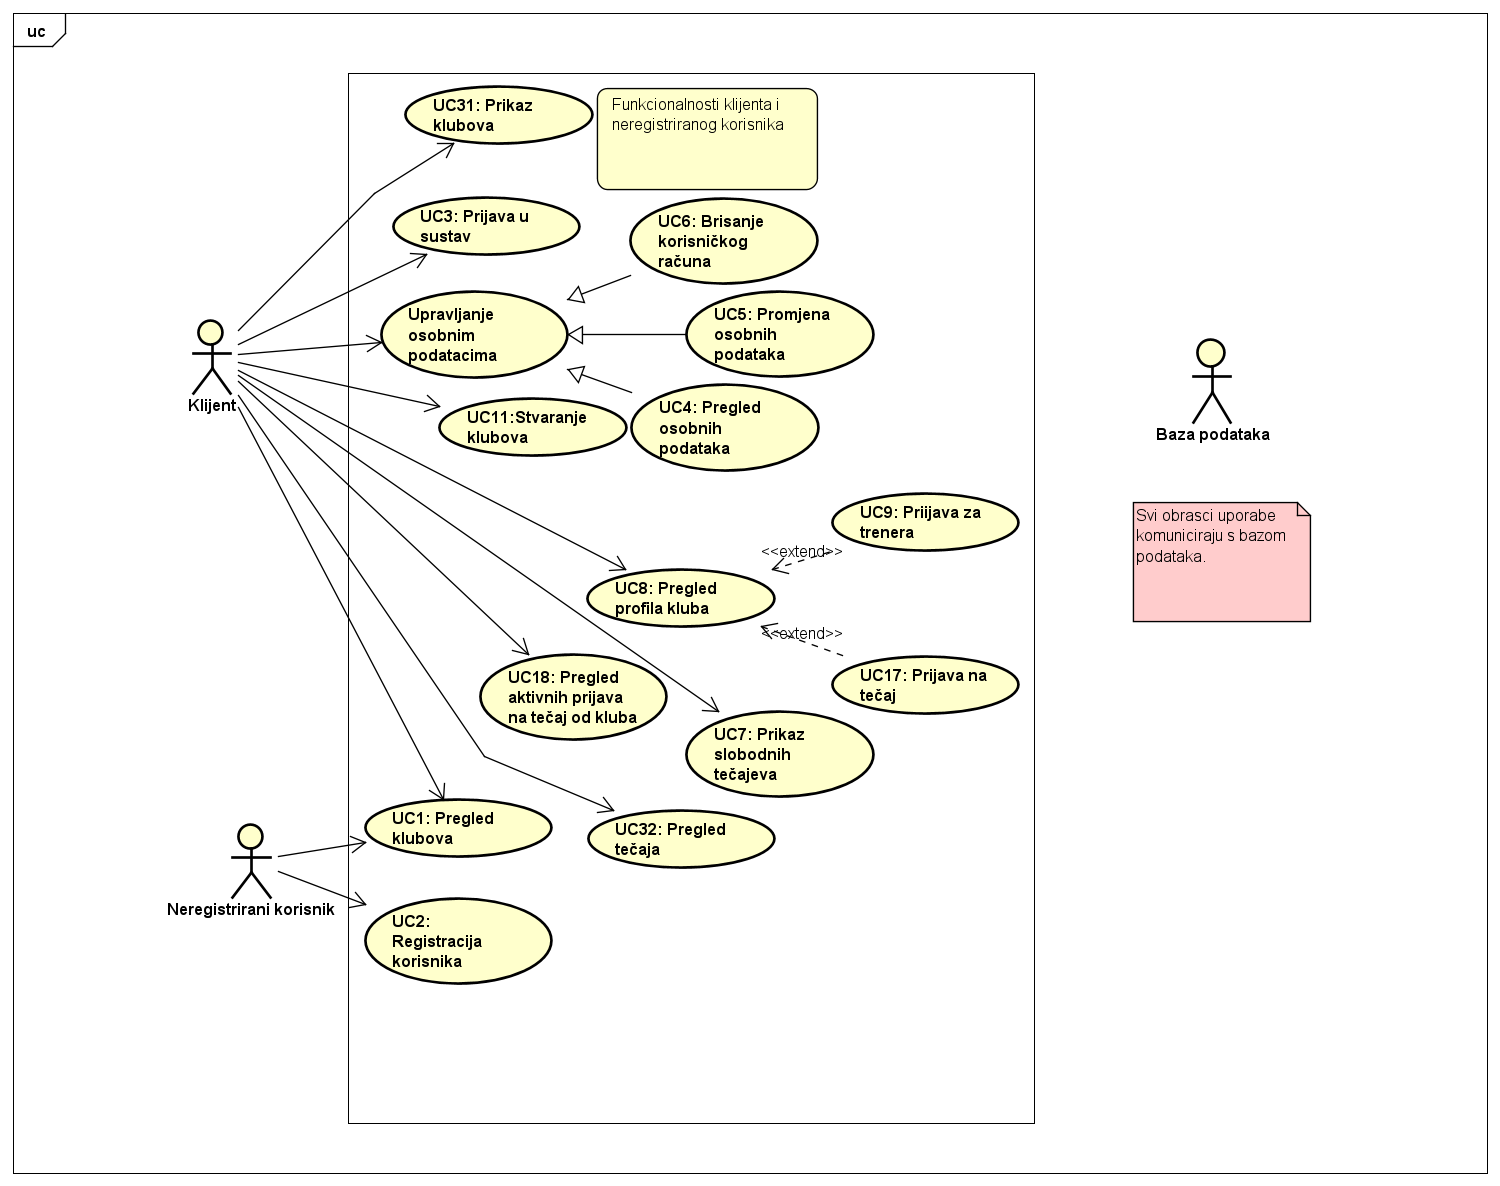
\includegraphics[width=\textwidth]{slike/Diagram1.png}
						\caption{Dijagram obrasca uporabe, funkcionalnost neregistriranog korisnika, klijenta i kluba}
						\label{fig:my_label}
					\end{figure}
					\begin{figure}[H]
						\centering
						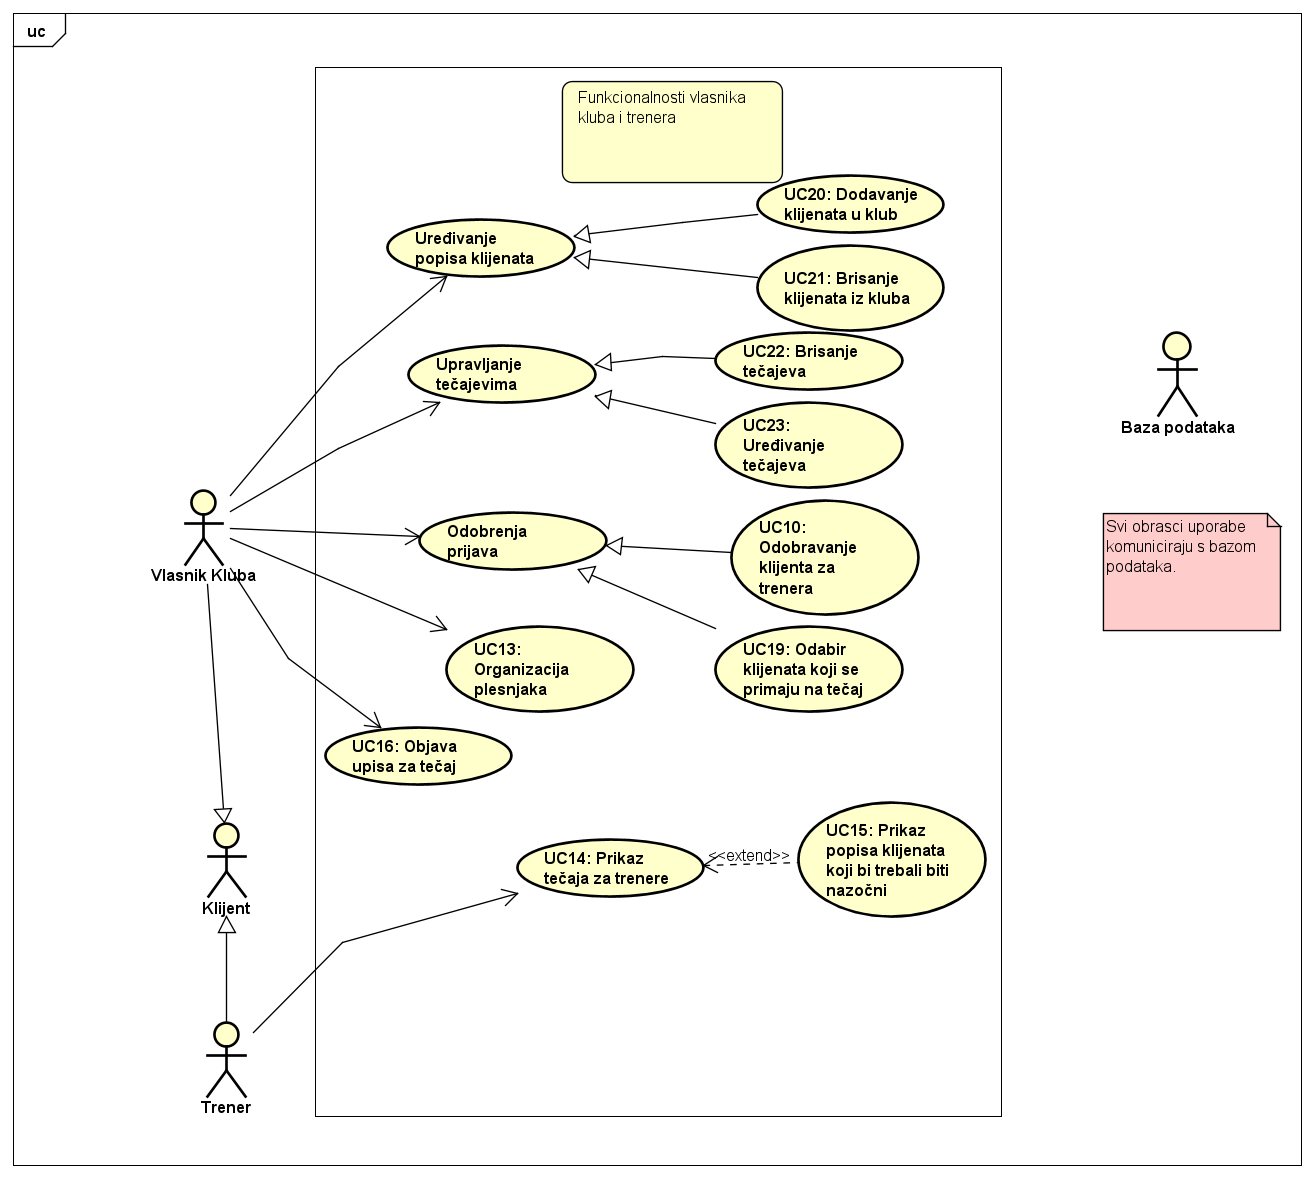
\includegraphics[width=\textwidth]{slike/Diagram2.png}
						\caption{Dijagram obrasca uporabe, funkcionalnost trenera i kluba}
						\label{fig:my_label}
					\end{figure}
					\begin{figure}[H]
						\centering
						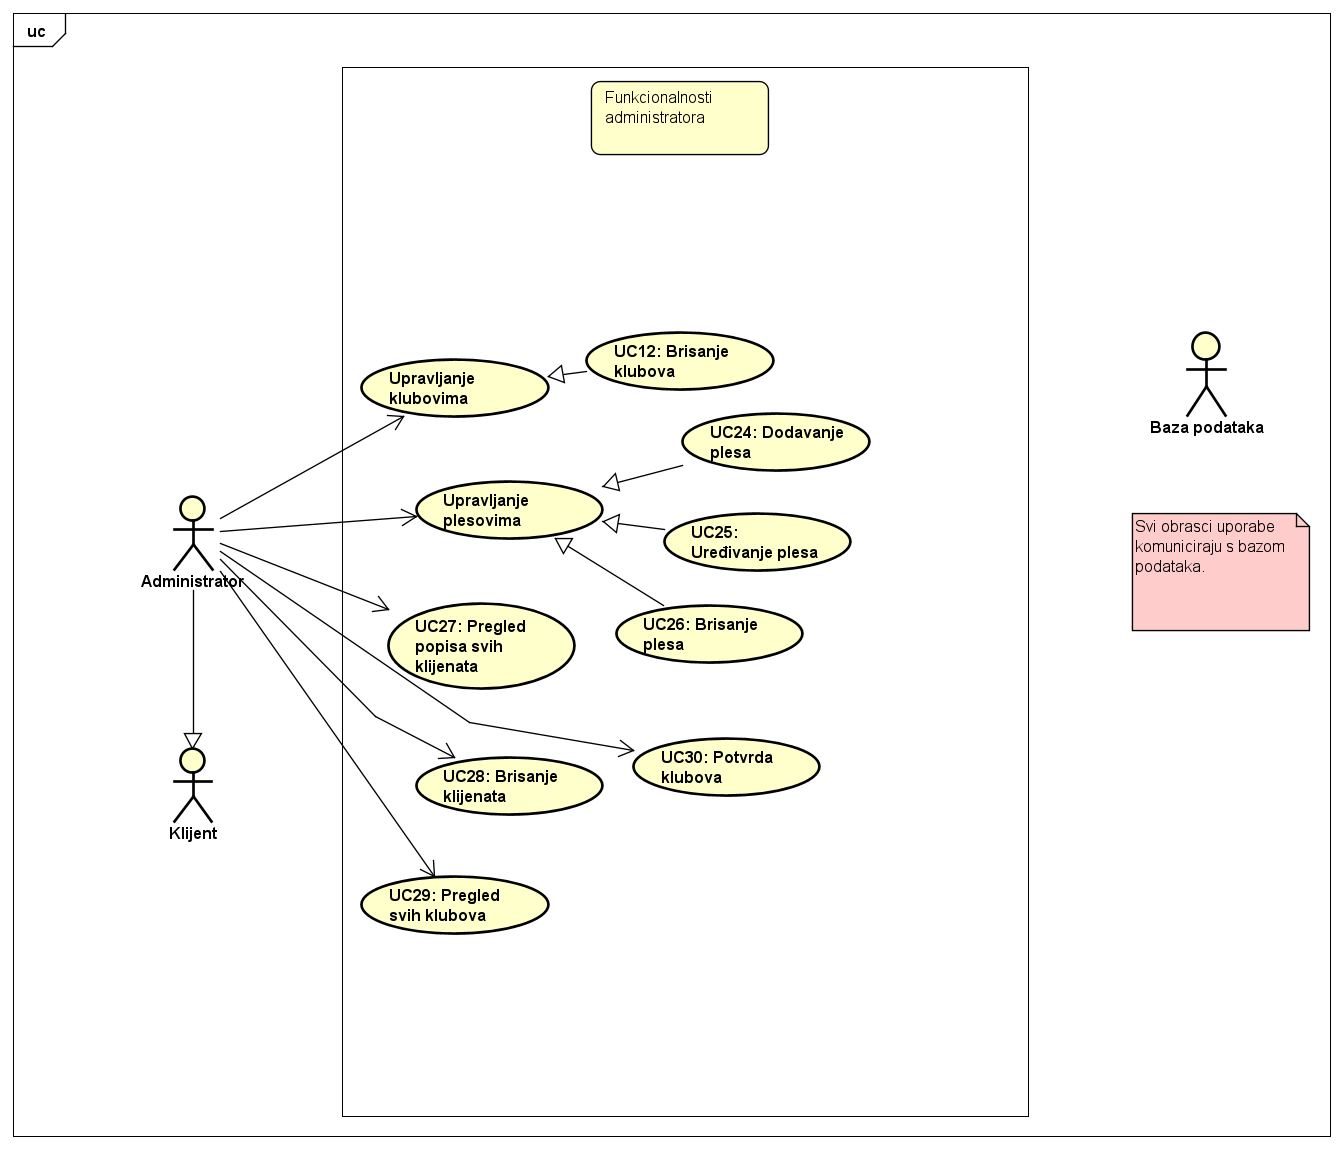
\includegraphics[width=\textwidth]{slike/Diagram3.png}
						\caption{Dijagram obrasca uporabe, funkcionalnost administratora}
						\label{fig:my_label}
					\end{figure}
			
			\eject
			\subsection{Sekvencijski dijagrami}
				
				\textbf{Obrasci uporabe: U31-prikaz klubova, UC8-Pregled profila kluba, UC9- prijava za trenera}\\
				
				Klijent šalje zahtjev za prikaz karte kako bi mogao odabrati klub.
				Poslužitelj dohvaća trenutne klubove i prikazuje ih. Odabirom kluba, poslužitelj iz baze podataka dohvaća osnovne podatke o klubu i prikazuje ih korisniku. Klijent odabire opciju prijave trenera. Poslužitelj isporučuje formu koja od korisnika traži predaju motivacijskog pisma i potvrde. Klijent predaje potrebne dokumente te prima poruku o uspješnoj pohrani prijave.
				
				\begin{figure}[H]
					\centering
					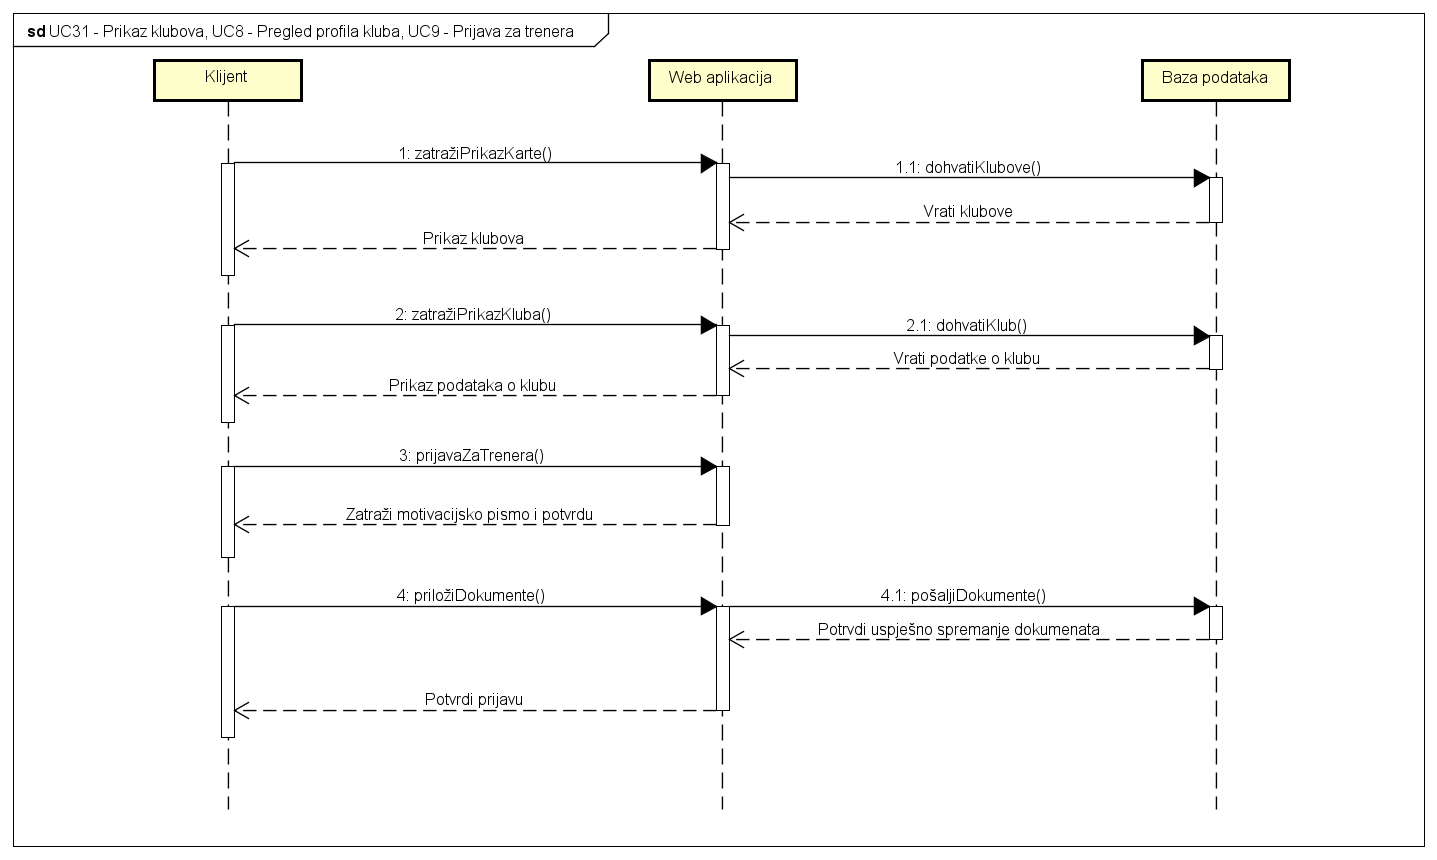
\includegraphics[width=\textwidth]{slike/seq_dijagram1.png}
					\caption{Sekvencijski dijagram za UC31, UC8 i UC9}
					\label{fig:my_label}
				\end{figure}
				\eject
				\textbf{Obrasci uporabe: UC7-prikaz tečajeva, UC32-Pregled tečaja, UC19- Odabir klijenta koji se primaju na tečaj}\\
			
				Vlasnik kluba šalje zahtjev za prikaz karte kako bi mogao odabrati tečaj. Poslužitelj dohvaća trenutne tečajeve i prikazuje ih. Odabirom tečaja, poslužitelj iz baze podataka dohvaća osnovne podatke o tečaju i prikazuje ih korisniku (vlasniku kluba). Vlasnik kluba odabire opciju pregleda prijava na tečaj. Poslužitelj dohvaća trenutne prijave na odabrani tečaj te ih prikazuje. Vlasnik kluba bira koje će klijente odabrat u grupu za tečaj. Pošlužitelj podatke o odabranim klijentima sprema u bazu. Pri završetku rada poslužitelj briše trenutne prijave iz baze.
			
				\begin{figure}[H]
					\centering
					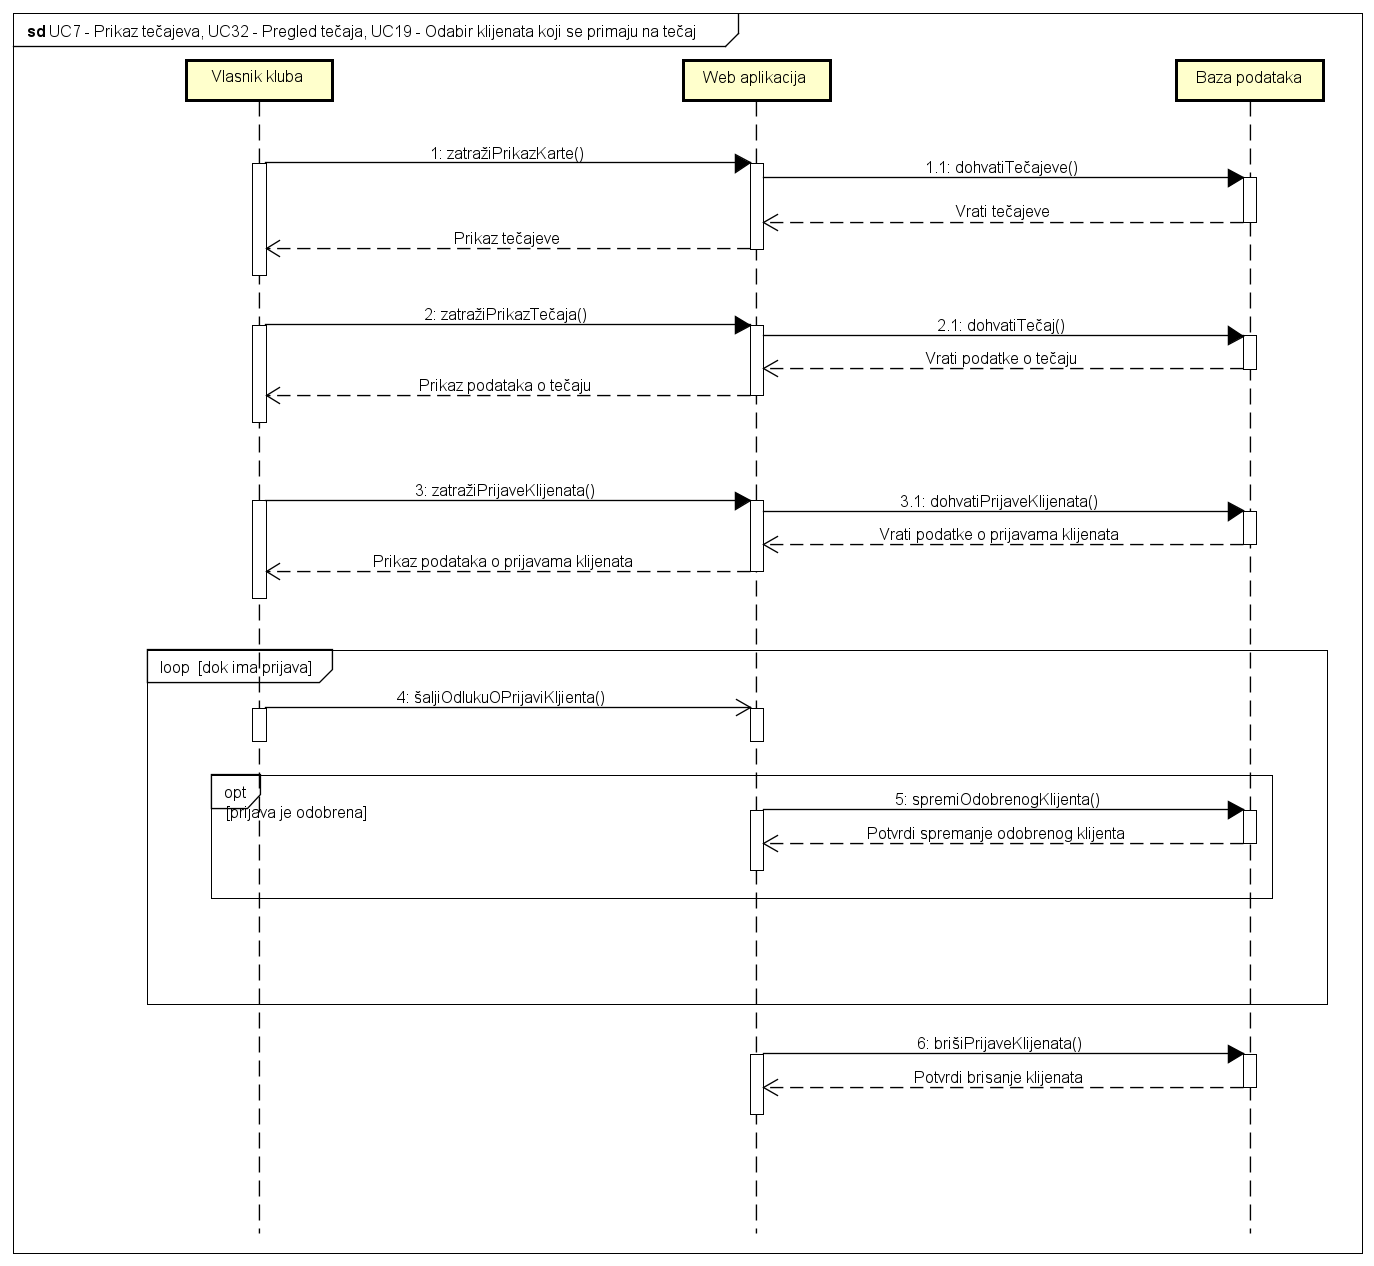
\includegraphics[width=\textwidth]{slike/seq_dijagram2.png}
					\caption{Sekvencijski dijagram za UC7, UC32 i UC19}
					\label{fig:my_label}
				\end{figure}
			\bigskip
			
				\textbf{Obrasci uporabe: UC13 - Organizacija plesnjaka}\\
				
				Vlasnik kluba šalje zahtjev za prikaz popisa svih dostupnih plesnjaka. Poslužitelj potom dohvaća sve dostupne plesnjake iz baze podataka i prikazuje ih korisniku (vlasniku kluba). Odabirom opcije dodavanja plesnjaka poslužitelj isporučuje formu koja od vlasnika kluba traži unos informacija za novi plesnjak. Vlasnik kluba ispunjava formu s potrebnim informacijama koje onda poslužitelj sprema u bazu podataka. Nakon spremanja poslužitelj zahtjeva od vlasnika kluba potvrdu o spremanju.
				
				\begin{figure}[H]
					\centering
					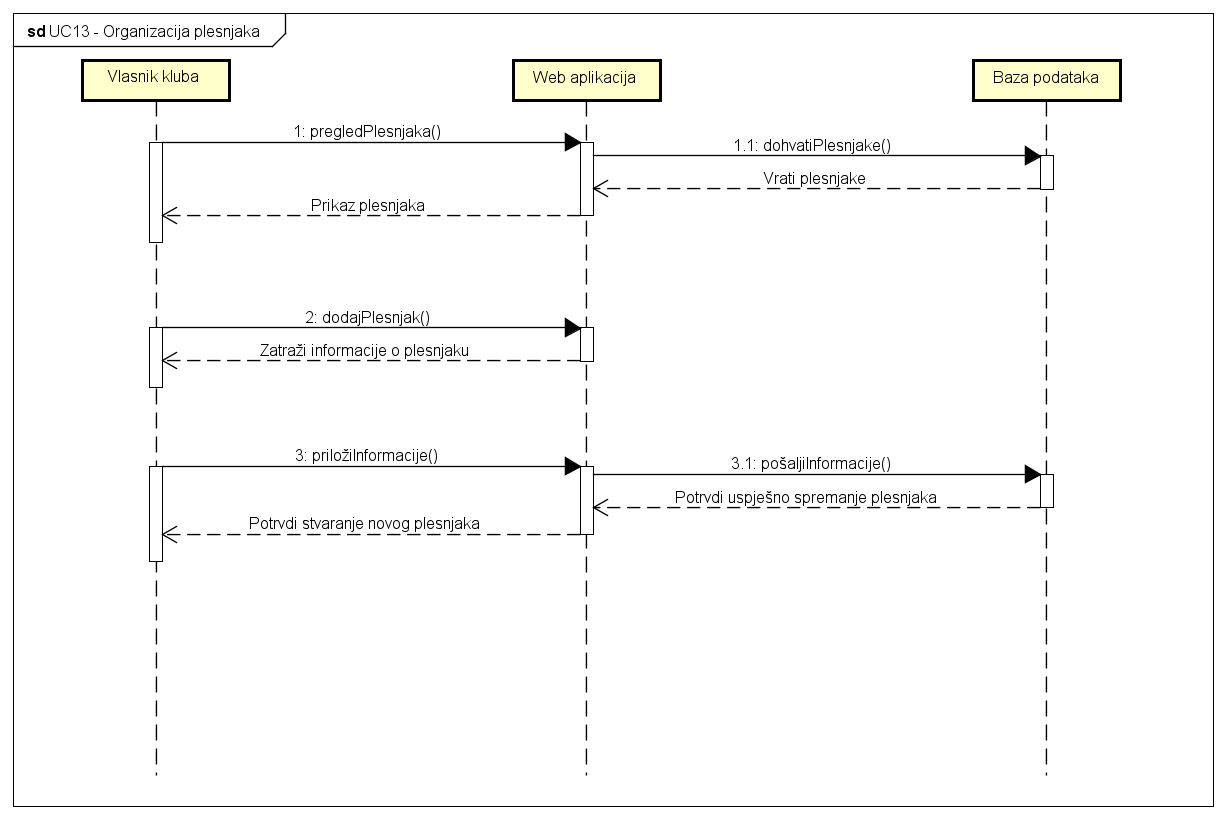
\includegraphics[width=\textwidth]{slike/seq_dijagram3.png}
					\caption{Sekvencijski dijagram za UC13}
					\label{fig:my_label}
				\end{figure}
			
		\newpage
			
				\textbf{Obrasci uporabe: UC11 - Stvaranje klubova, UC30 - Potvrda klubova}\\
				
				Klijent šalje zahtjev za stvaranjem novog kluba. Poslužitelj potom isporučuje formu koja od klijenta  traži informacije za novi klub. Popunjavanjem forme poslužitelj sprema informacije o novom klubu u bazu podataka te zatim traži od klijenta potvrdu o stvaranju istog. Administrator šalje zahtjev za potvrđivanje klubova. Poslužitelj iz baze podataka dohvaća popis svih nepotvrđenih klubova i prikazuje ih administratoru sustava. Sve dok postoje nepotvrđeni klubovi administrator šalje odluku hoće li određeni klub odobriti ili ne. Ako je klub odobren, poslužitelj tu informaciju sprema u bazu. Ako je administrator potvrdio klub klijent koji je poslao zahtjev postaje vlasnikom kluba. Na kraju poslužitelj briše zahtjeve iz baze.
				
				\begin{figure}[H]
					\centering
					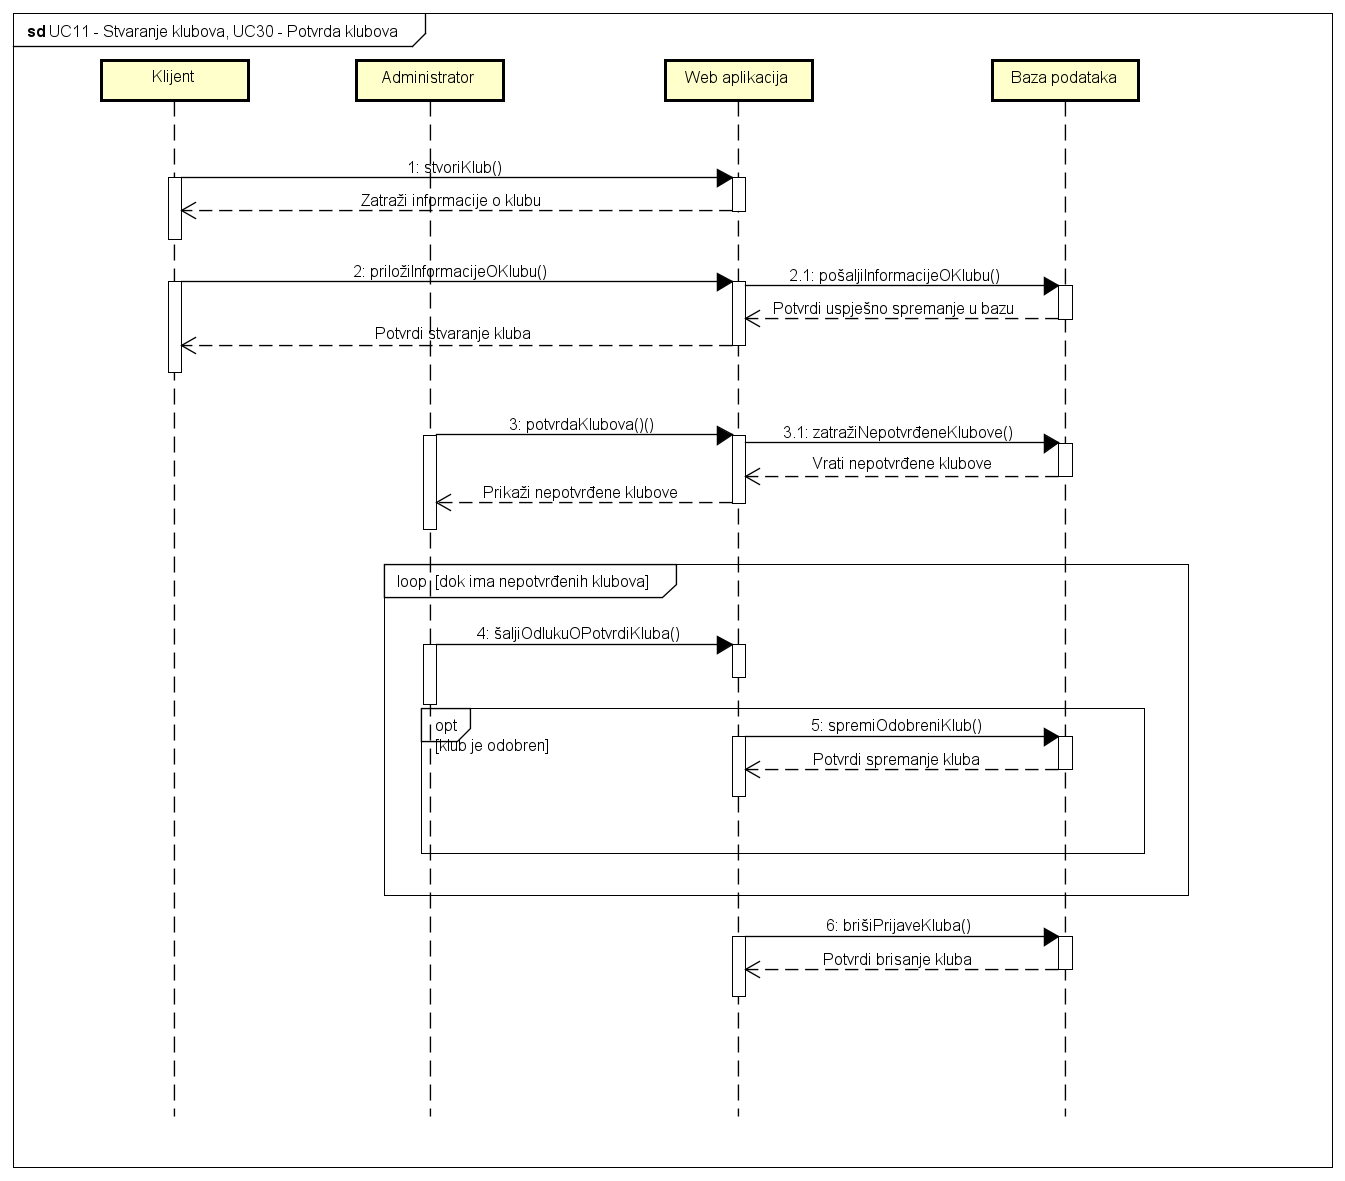
\includegraphics[width=\textwidth]{slike/seq_dijagram4.png}
					\caption{Sekvencijski dijagram za UC11, UC30}
					\label{fig:my_label}
				\end{figure}
	
		\section{Ostali zahtjevi}
		
		
			 \begin{packed_item}
			 	\item {Sustav mora omogućiti rad više korisnika u stvarnom vremenu}
			 	\item {Sustav treba kriptirati password koji korisnik unosi}
			 	\item {Veza s bazom podataka mora biti kvalitetno zaštićena te brza i otporna na vanjske greške}
			 	\item {Izvršavanje dijela programa koji pristupa bazi podataka ne smije trajati duže od par sekundi}
			 	\item {Korisničko sučelje i sustav moraju podržavati hrvatsku abecedu pri unosu i prikazu tekstualnog sadržaja}
			 	\item {Sustav treba biti implementiran kao web aplikacija koristeći objektno-orijentirane jezike}
			 	\item {Sustav mora biti lagan i intuitivan za korištenje, kako bi ga koristili korisnici bez dodatnih opširnih uputa}
			 	\item {Nadogradnja sustava ne smije narušavati postojeće funkcije sustava}
			 	\item {Neispravno korištenje korisničkog sučelja ne smije narušiti funkcionalnosti i rad sustava}
			 \end{packed_item}
			 
	